\clearpage
\section{Configuring ROS for mapping}

During the installation of ROS on Ubuntu, a new package named Hector-slam was discovered. This package allows ROS to generate a map without the use of the GMapping package, which was one of the packages that caused issue during the installation process on Raspbian. Its biggest advantage is that it does not rely on odometry to know whether the reference frame has changed. Odometry is the use of data from sensors to estimate the difference in position over time. It is used by robotic systems to estimate their position relative to a starting point. It is also important to highlight that is does not determine, but estimates this position in space and time.

\subsection{How ROS works}
During our development, we gained a deep understanding of how all the moving parts in ROS work well together. The following diagram showcases the general flow of how the ROS system that we built up works.

\begin{figure}[H]
	\centering
	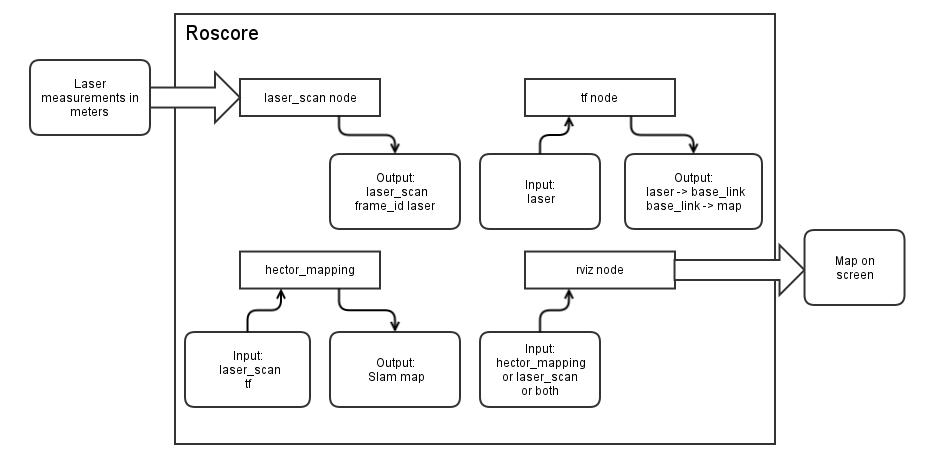
\includegraphics[width=1\linewidth]{images/ROSflow.png}
	\caption{ROS flow diagram, showcasing the map generation from sensory readings}
\end{figure}

\textbf{Roscore} is the main process behind ROS and it allows for all running nodes to talk to each other, although by itself it does nothing, just keeps running in the background.

Nodes are the smallest parts of ROS that are put together to form a full application. They are run as separate processes, all with their own executable files. The only way nodes communicate is through the roscore. To make a node, it is necessary to use or create a ROS library, written in any desired programming language.

\textbf{Roslaunch} is the ROS command that allows starting multiple nodes, and also allows giving parameters to nodes. Roslaunch executes nodes that are specified in an XML file you give it, called the launchfile.

\textbf{Bagfiles} are used for storing ROS message data, transmitted over any topic visible to list by calling \textit{rostopic list} command. Bags are typically created by a tool like rosbag, which is subscribed to one or more ROS topics, and store the serialized message data in a file as it is received. These bag files can also be played back in ROS to the same topics they were recorded from, or even remapped to new topics. Once the current node setup has been established and the correct information is transmitted over the topics, the data will be stored in a .bag file.

\subsection{Developing for ROS}
During this stage of development, the gathering of the data happens on the Raspberry Pi, while a map is generated using ROS. The Raspberry Pi is accessed through SSH and the generated map is then broadcasted to another computer through that SSH connection, for visualization the tool called rviz is used. 

To achieve this, we had to set up a direct connection between one of our developer computers running Ubuntu and the Raspberry Pi using a CAT5 Ethernet cable. Then we created a new network settings, set the IPv4 method to be 'Shared to other computers' which bridged the two network adapters and transmitted internet access to the Raspberry Pi from our own computers, connected to the internet via Wi-Fi. Then we located the leases and found the IP address assigned to the connected device. To connect via ssh we used the following command line:
\lstset{language=sh}
\begin{lstlisting}
	>> $ ssh -Y username@ip-address
\end{lstlisting}
This enabled us to connect to the Raspberry and by using the \textit{-Y} flag, it allowed us to stream the graphical application using X11 forwarding.

Although, this seemed to be working quite well, this operation required quite a lot of memory and processing power, therefore some issues were experienced:

\begin{figure}[H]
	\centering
	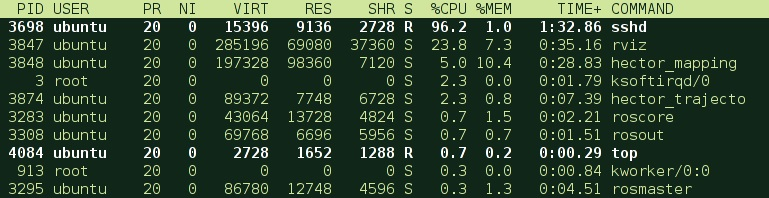
\includegraphics[width=.8\linewidth]{images/rvisScreenshotCropped.jpg}
	\caption{The resource usage}
\end{figure}

Looking at the figure above, we can observe several things by running the mapping operation: by generating the actual map directly on the Raspberry Pi required too many resources from the CPU, and that the rendering of the visualization tool, rviz, channeled through the SSH connection to the computer screen required more bandwidth than there could be supplied. This caused a terrible lag and a bad experience both for us developing, but for the end result too.

To reduce the amount of resources used by the Raspberry Pi, the map needs to be generated and visualized using separate computing unit. ROS is built to have separate nodes with a main computing unit.

To copy files to and from the Raspberry, we used the \textit{scp} utility, and therefore no version control setup was not necessary on the controller. The command line was used to transfer .bag files and source code:
\begin{lstlisting}
	>> $ scp username@from-ip-address:~/file /home/mylocaluser/to-location/
\end{lstlisting}

When the custom laser node written by us, has been started, it starts publishing laser readings in form of a LaserScan message, to the \textbackslash\textit{scan} topic. By using the following command, we could listen to it and see the outcome of our scanning:

\lstinputlisting[firstline=1, lastline=17, language=C++]{../code/sampleOutput.txt}

As the output shows, the number of readings is being stored in an array that is published to \textbackslash scan and then used by ROS to visualize or transform it later on. These readings are represented in a floating-point number in meters. Range is also represented in meters, but they are hard-coded, as the minimum and maximum value of the range does not change, but rather set by the manufacturer. The messages are time-stamped, which turned out to be very important when ROS transforms them for mapping and there is also a scan time, which tells the time between the scans in seconds. The angle values are radians of the start and end angle of the scan, while the angle increment is the angular distance between measurements. Our laser does not provide intensity-data, therefore we did the array has been left empty.

With this, we set up everything for starting to create a map in 2D using Hector-slam.